% Asset ID: AS1VectorsTikZ-002
% Source: P1-Chp11-Vectors.pdf, Triangle Law for vector addition
% Related lesson section: Core Theory: Vector addition; Worked Example 1
% Purpose: Illustrate the triangle law AB + BC = AC and the resultant vector.
\documentclass[tikz,border=8pt]{standalone}
\usepackage{amsmath}
\usepackage{bm}
\usetikzlibrary{arrows.meta,positioning,angles,quotes}
\begin{document}

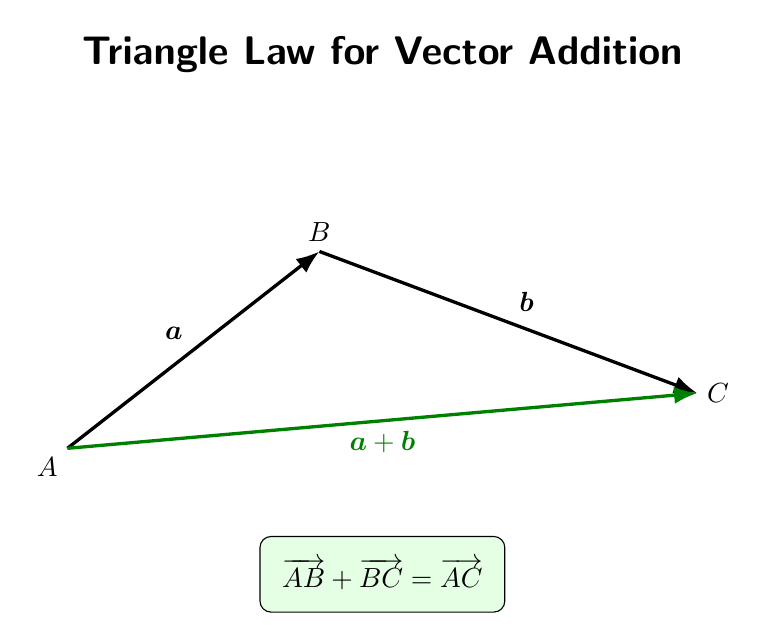
\begin{tikzpicture}[>=Latex,every node/.style={font=\sffamily},vector/.style={->,very thick},result/.style={->,very thick,green!50!black}]
\node[font=\sffamily\bfseries\Large] at (0,4) {Triangle Law for Vector Addition};
\coordinate (A) at (-4,-1);\coordinate (B) at (-.8,1.5);\coordinate (C) at (4,-.3);
\draw[vector] (A)--node[above left] {$\bm a$}(B);
\draw[vector] (B)--node[above right] {$\bm b$}(C);
\draw[result] (A)--node[below] {$\bm a+\bm b$}(C);
\node[below left] at (A) {$A$};\node[above] at (B) {$B$};\node[right] at (C) {$C$};
\node[draw,rounded corners,fill=green!10,inner sep=8pt] at (0,-2.6) {$\overrightarrow{AB}+\overrightarrow{BC}=\overrightarrow{AC}$};
\end{tikzpicture}

\end{document}
